\documentclass[14pt]{book}
\usepackage{graphicx}
\usepackage{ngerman}
\usepackage[latin1]{inputenc}

\title{Spiel Konzept}
\author{Maik W"ohl}
\date{\today}

\begin{document}
\maketitle

\tableofcontents

\chapter*{Vorwort}

Ich habe noch keinen Namen f"ur dieses Spiel aber ich habe mir mal gedacht ein HTML5 Rollenspiel zu basteln, dass eine isometrische 2D Grafik bietet. Nat"urlich, dachte ich, brauche ich daf"ur auch eine Engine oder eher JS-Bibliothek die mir da einiges an Schreibarbeit sp"ater abnimmt und habe viel gesucht und leider nichts passendes gefunden. Das hei"st f"ur mich, dass ich die Engine selber schreiben muss.

Ich habe mir auch schon f"ur die Spielumsetzung einiges ausgedacht. Aber dazu sp"ater mehr. Ich habe zum Beispiel schon ein Logo f"ur meine GitHub Organisation \textbf{DaemonArtStudios}. Hier ist es:

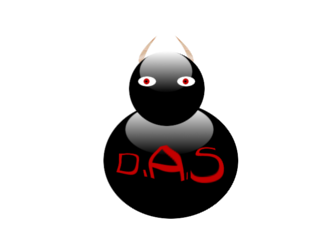
\includegraphics{logo-das-small}

\part{Vorstellung}

\chapter{Spielidee}

Dieses Spiel soll kein MMORPG werden, das hei"st es beherrscht nur einen Einzelspieler-Modus. Der Kamerawinkel auf das Geschehen sollte in einem Winkel wie in \emph{Pokemon} oder \emph{Secret of Mana} auch benutzt wird, eingestellt sein. Man wird direkt in das Geschehen reingeworfen, eiskalt. Das hei"st man muss sich die Steuerung selber aneignen, und das tut man, indem Hinweisboxen zur jeweiligen Situation auftauchen und einem helfen. Sollte man diese nicht mehr ben"otigen, kann man diese auch abschalten.

Da das ganze im Einzelspieler-Modus gehalten ist, muss die Story packend sein, weil beim Multiplayer die anderen Spieler und die Gemeinschaft auch eine Rolle spielen, wie lange sich der Benutzer mit dem Spiel besch"aftigt.

Wechselkurse f"ur Geld und andere "ahnliche Dinge und auch die Verkaufwerte von Gegenst"anden sollen zentral geregelt werden und mit jedem Spielstart aktualisiert werden. 
 

\chapter{Spielumsetzung}

Dieses Spiel wird ein Browser-Spiel werden, was die neue Technologien verwendet. Diese sind also folgend im Namen HTML5 zusammengefasst. Man wird wegen der Inkompatiblit"at zu "alteren Browsern keinen Polyfill einsetzen m"ussen, da das Spiel nur auf modernste Browser setzt.

Das Spiel wird keinen Server ben"otigen, deswegen werden alle  zeitkritischen Daten wie die aktuellen Wechselkurse f"ur das Geld nicht im \emph{ApplicationCache} vorgehalten und bei jedem Spielstart aktualisiert. Das ist sehr ungew"ohnlich f"ur ein Einzelspieler RPG, aber das macht grade den Reiz aus, der dem Spieler vermittelt werden soll. Aktuelle reale Wechselkurse f"ur das Geld und f"ur jeden Spieler gleiche Verkaufswerte in Markthallen und bei H"andlern.

Vielleicht wird auch ein Server implementiert, der alle Daten synchronisiert und wenn sich der Spieler bei einem anderen Computer einloggt sollen die Daten wie Inventar und Bankinhalt auf den Computer transferiert werden. Das steht aber noch nicht fest und ist auch ein optionales Feature. Als andere L"osung k"onnte man auch ein Export-Format entwickeln, dass es einem erm"oglicht alle relevanten Daten zu exportieren und dieses \emph{Benutzerprofil} wieder zu importieren.


\part{Detaillierte Beschreibung}

\chapter{Kommunikation und Interaktion}

Die Kommunikation in einem Spiel ist mitunter das wichtigste. Hier sollte die Kommunikation "uber Schl"usselw"orter im Dialog und per Chat-Eingabe verlaufen. Hier sieht man gewissen Parallelen zum Spiel \emph{Tibia}. 

\section{NPC's}

NPC's sind sogenannte \emph{Non Player Character's} welche computergenerierte Objekte sind. Diese erhalten einen klar strukturierten Wortschatz der aber erweiterbar ist. Wenn man einem NPC etwas beibringt, so soll dieser in der Lage sein dieses Wissen oder diesen Zugriff zu behalten. Das soll "uber einen Key-Value Store/LocalStore erm"oglicht werden. In diesem KVS werden die Namen im Schema \emph{NPC:Aktion | Reaktion} festgehalten. Sollte der Spieler also das Schl"usselwort AKTION in den Chat schreiben und dabei in einem Satz den Namen des NPC sagen, so wird dieser mit einer REAKTION reagieren. Diese kann verschieden ausfallen. Man sollte lediglich die Lernf"ahigkeit dieses NPC's auf gewisse Vorg"ange beschr"anken k"onnen. Man soll sich sein eigenes RPG dadurch erschaffen, dass man z.B. einen Magier zu einem Teleporter umwandelt und eine Masse an KVS-Daten anlegt die einen z.B. zu einem Kooridinatenpunkt im Spiel teleportieren. Das gibt es in keinem Spiel und erfordert viel Arbeit.

\subsection{Chat}

Da der Chat nur f"ur die Kommunikation zwischen Spieler und NPC ben"otigt wird, erscheint dieser zentriert am unteren Rand des Bildes wo links mitte und rechts mitte die Gesp"rachspartner platziert sind. Vorz"uglich der Spieler am linken Rand. Hier k"onnen Standardanimationen angewandt werden.

\subsection{Aussehen}

Das Aussehen eines NPC's sagt meist viel "uber seine Funktion im Spiel aus, so soll ein Magier auch eine Tracht tragen und ein Bogensch"utze auch einen Bogen. Im Dialog sollten die 2D Elemente sichtbar sein. Da im 2D Context kein echtes 3D m"oglich ist, soll stattdessen die Berechnung des Canvas eingestellt werden, also der Inhalt gesichert und leer geschrieben werden und ein Video-Overlay daneben erscheinen bzw. wenn es die Technik erm"oglicht, das Video dar"uber zu legen. Ein Videosequenz wo bei einer Auswahl der Antwort aber dann doch per Maus gespielt werden muss. Hier sollten diese in einem Programm wie Blender oder Cinema 4D modelliert werden und eben als Video abgespeichert werden. Diese Art des Chats ist aber eher fortgeschritten und muss nicht unbedingt zum Einsatz kommen, es reicht auch die Kommunikatio "uber den Chat.

\section{Items und Spielobjekte}

Items und Spielobjekte die bspw. eine Aktion ausl"osen, wie etwa ein Heiltrank oder ein Portal sollten "uber den Chat bzw. "uber einen Shortcut erreichbar sein. Hier wird sich einem KeyDown Event bedient, ein entsprechender Keylogger ist leicht gebaut.

Items sollte in einer PNG-Grafik vorliegen die Alpha-Transparenz kennt, da die Items einmal gezeichnet werden und fortan nur als gr"o"sere oder kleinere Grafik erscheinen. Je nach Hintergrund verschieden.

\chapter{F"ahigkeiten}

Ein Charakter sollte entsprechende F"ahigkeiten haben. Diese werden nicht durch eine \emph{Rassenwahl} festgelegt, sondern durch den Spielverlauf. Der Spieler bestimmt, was er wird. Kann er gut mit Pfeil und Bogen so wird er Bogensch"utze. Das setzt aber auch ein Durchhalteverm"ogen und ein offenes Levelsystem voraus. 

\section{Shortcut-Leiste}

Die Shortcut-Leiste ist eine sich am unteren Bildrand befindende Leiste die es erm"oglicht "uber die Zahlen 1-0 auf F"ahigkeiten zuzugreifen, die dort abgelegt wurden. 

\section{Abh"angigkeiten}

Jede F"ahigkeit sollte Abh"angigkeiten besitzen. Diese Abh"angigkeiten k"onnen aus Heiltr"anken oder anderen Items bestehen. Ein Heilzauber sollte je nach Stufe entsprechende Mengen an Heiltr"anken oder Pflanzen voraussetzen. 

\section{M"ogliche F"ahigkeiten}

Es sollte verschiedene F"ahigkeiten f"ur die gew"ahlte prim"are Waffe geben. Das k"onnen nicht nur Zauber sein sondern auch Bewegungsk"unste wie das schnelle Ausweichen oder der Sprung "uber den Gegner mit anschlie"sendem Erstechen von hinten. Solche Sachen sollten m"oglich sein.

\end{document} 

